
\فصل{مفاهیم پایه و نحوه کارکرد شبیه‌ساز}


\section{مفاهیم پایه}



در ابتدا به طور مختصر به مفاهیم پایه مورد استفاده در این پروژه می‌پردازیم.

همان طور که در مقدمه گفته شد، قرار است با یک
 \lr{k-ary n-cube}
 کار کنیم. نام دیگر این شبکه توری مدور \LTRfootnote{Torus} است و شبکه‌ای است که از نظر طراحی کلی، به شدت شبیه شبکه توری عادی \LTRfootnote{Mesh} است با این تفاوت که رئوس ابتدا و انتهای هر بعد هم به یکدیگر متصل هستند و عملا در هر بعد یک حلقه \LTRfootnote{Ring} را ایجاد می‌کنند. در این توپولوژی،‌ n نشان‌دهنده تعداد ابعاد و k نشان‌دهنده تعداد گره در هر بعد است. باید توجه کرد که Torus به شکل کلی می‌تواند در هر بعد گره‌های متفاوتی داشته باشد ولی
  \lr{k-ary n-cube}
 شکل خاصی از Torus است که همه بعد‌های آن اندازه یکسانی دارد. یک نمونه از آن را در شکل \ref{fig:torus} 
 مشاهده می‌کنید.
 
 

 \شروع{شکل}[ht!]
 \centering
 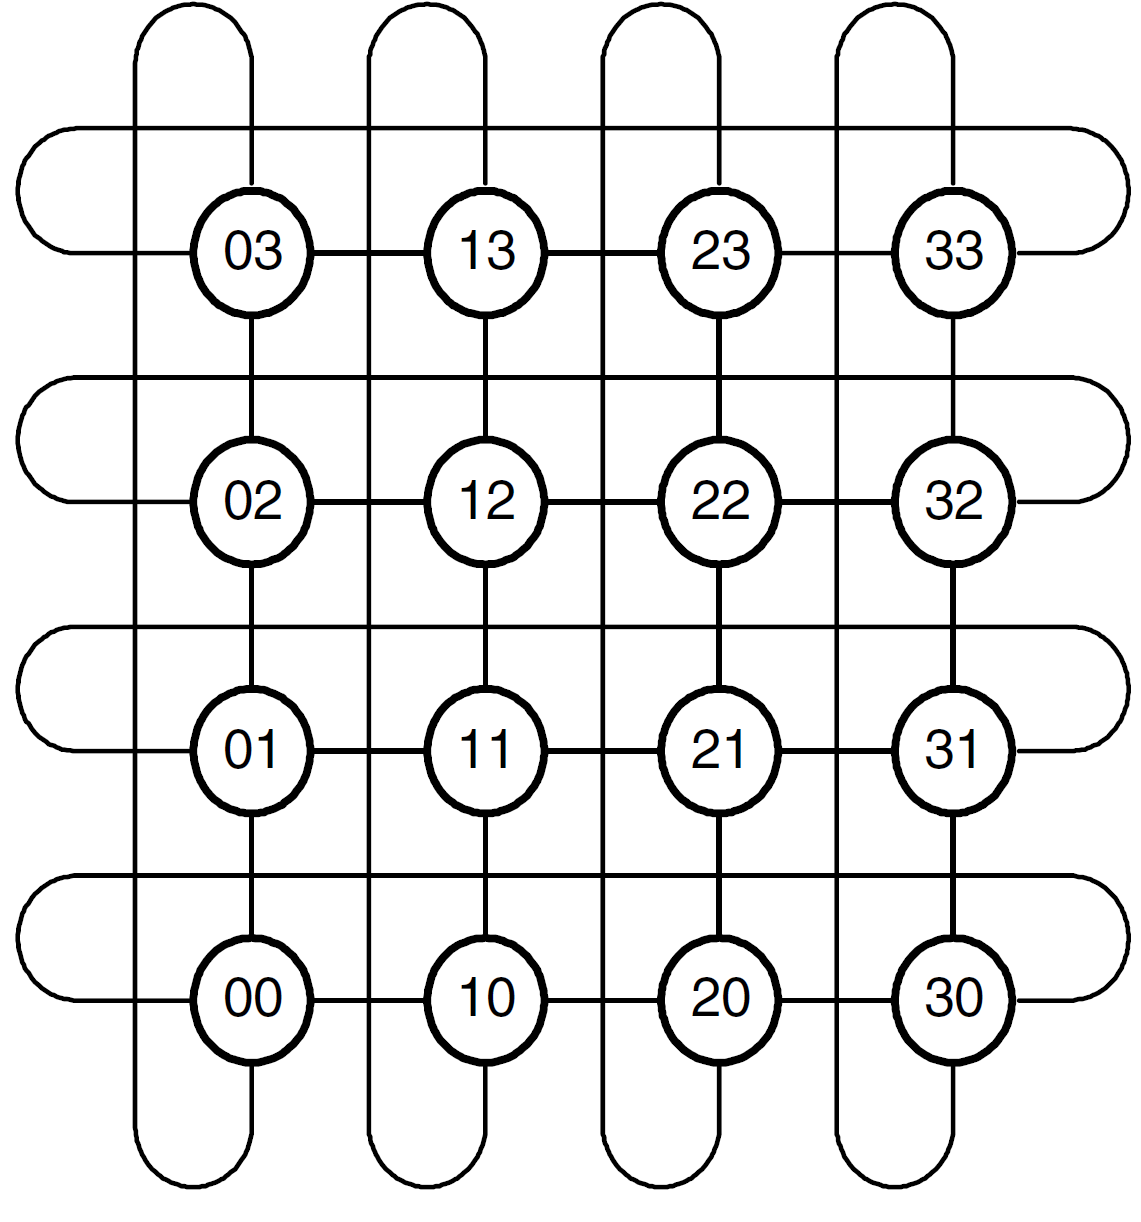
\includegraphics[width=0.4\textwidth]{Torus2.png}
 \شرح{یک 
\lr{4-ary 2-cube} 
}
 \label{fig:torus}
 \پایان{شکل}

 
 



از جمله ویژگی‌های مهم \lr{k-ary n-cube} می‌توان به موارد زیر اشاره کرد:

\begin{itemize}
	\item
	سایز شبکه: $k^n$
	
	\item
	درجه رئوس: $n$
	
	\item 
	قطر: $n(k-1)$
	
	\item 
	منظم‌ است.
	
	\item 
	متقارن است.
	
	\item
	درجه اتصال:
	$\frac{n}{k^n -1}$
	
	\item 
	عرض برشی:
	$\frac{k^n}{k} = k^{n-1}$
	
	
	
\end{itemize}


مسئله دیگر، مسیریابی \lr{Duato} است. به طور کلی ما علاقه‌داریم که درجه \lr{Adaptivity} الگوریتم مسیریابی ما بالا باشد تا سیستم ما کارایی بالاتری داشته باشد. در شبکه‌های
\lr{ Fully Adaptive} امکان استفاده از همه کانال‌ها وجود داشته و درجه \lr{Adaptivity} برابر ۱ می‌شود. با این حال مشکلی که وجود دارد این است که ممکن است الگوریتم ما امکان بن‌بست داشته باشد. بن‌بست به معنی وابتسگی حلقوی چندین گره به هم برای عبور پیام است و در این صورت هیچ کدام امکان آن را نخواهند داشت. با این حال می‌دانیم تعدادی الگوریتم \lr{Deadlock Free} هم وجود دارند که نبود بن‌بست را تضمین می‌کنند. با این وجود پرفرمنس این الگوریتم‌ها لزوما خوب نیست.


روش \lr{Duato} به این صورت است که تعدادی کانال مجازی به منظور اجرای یک الگوریتم \lr{Deadlock Free} قرار می‌دهد و از سایر کانال‌های مجازی پیام‌ها با یک الگوریتم \lr{Fully Adaptive} بهینه عبور داده می‌شوند. در صورتی که در قسمتی از کار متوجه بن‌بست شدیم، پیام به کانال‌های مجازی که به منظور انتقال پیام‌ها به صورت \lr{Deadlock Free} تعیبه شده‌اند منتقل شده و با الگوریتم آن قسمت انتقال خود را انجام می‌دهد. به این ترتیب ما هم می‌توانیم از مزایای الگوریتم‌های سریع \lr{Fully Adaptive} که لزوما تضمین برای نبود بن‌بست نمی‌دهند استفاده کنیم و هم از مزایای الگوریتم‌هایی که به ما تضمین می‌دهند بن‌بستی وجود نخواهد داشت.



\section{نحوه کارکرد شبیه‌ساز}


شبیه‌ساز \lr{Booksim} شبیه‌ساز قدرت‌مندی است که بسیاری از نیازهای مربوط به شبیه‌سازی شبکه‌های میان‌ارتباطی در آن پیش‌بینی شده است. از پیاده‌سازی الگوریتم‌های مختلف مسیریابی گرفته، تا توپولوژی‌های مختلف و حتی ریزمعماری روترها. این ساختار به شکلی کاملا \lr{Modular} طراحی شده و برای تغییر در یک قسمت خاص نیازی نیست که در سایر قسمت‌ها تغییر بزرگی ایجاد بشود.


علاوه بر این،‌ شبیه‌ساز \lr{Booksim} ساختار خاصی برای فایل‌های \lr{Config} خود دارد و براساس ساختار این فایل‌ها اقدام به شبیه‌سازی شبکه می‌کند. در زیر نمونه‌ای کوچک از ساختار یک فایل \lr{Config} آمده است.


\begin{latin}
	
	\begin{verbatim}
		// Topology
		topology = torus;
		k = 16;
		n = 2;
		// Routing
		routing_function = dim_order;
		// Flow control
		num_vcs = 4;
		// Traffic
		traffic = uniform;
		injection_rate = 0.3;
		sim_type = throughput;
	\end{verbatim}
\end{latin}

در ساختار بالا، \verb*|topology| مشخص کننده نوع توپولوژی و مقادیر \verb*|k| و \verb*|n| مشخص کننده پارامترهای آن هستند. \verb*|num_vcs| نشان‌دهنده تعداد کانال‌های مجازی است. \verb*|traffic| نشان‌دهنده نوع ترافیک ورودی، \verb*|injection_rate| نرخ ورود بسته‌ها و در نهایت \verb*|sim_type| مشخص می‌کند که پردازش‌ها متمرکز بر نرخ تاخیر باشد یا \lr{throughput}.

در بین فایل‌های اصلی که در این پروژه وجود دارد، فایل‌های پوشه \verb*|routers| برای شبیه‌سازی \lr{Router} ها بوده و فایل‌های پوشه \verb*|networks| تعریف‌کننده انواع توپولوژی‌هاست. همچنین فایل \verb*|routerfunc| مربوط به الگوریتم‌های مسیریابی‌ مختلف است. عمده تغییرات ما مربوط به \verb*|routerfunc|  خواهد بود.




